\section{Pattern Matching in Hazel}\label{sec:examples}
\todo{Make sure this section uses consistent wording with the rest of the paper (e.g. case vs. match, branch vs. rule, indeterminate) - if using match should probably have footnote or something saying we call it case in Hazel}
Let us begin with some examples to develop the intuition for pattern matching with typed holes.
Our examples are shown in the implementation in Hazel.

Suppose a programmer is writing a function \texttt{has\_odd\_length} which should take in a list of \texttt{Int}s and result in a \texttt{Bool} indicating if that list has an odd number of elements. 

First we will build the intuition for exhaustiveness checking when there are holes in the patterns of a match expression. 
When there are holes, we consider if there is a way that the holes \emph{could} be filled such that the match expression would be exhaustive. 
If there is, we say that the match expression may or may not be exhaustive because we do not know if the holes will be filled with one of the exhaustive hole fillings or if a non-exhaustive hole filling will be used. 
If there is no way to fill the holes such that the match expression would be exhaustive, then we say that the expression must not be exhaustive. 

Let us look at \autoref{fig:exhaustiveness} for an example of exhaustiveness checking using our \texttt{has\_odd\_length} function. 
We see in \autoref{fig:may-exhaustive} that the pattern of the second branch of the match expression contains a hole.\todo{Should probably indicate that you don't need to worry about the numbers other than just considering them as identifiers}\footnote{In the Hazel UI, hole numbers are shown as light grey text inside the hole. } 
This hole could be filled in such that the match is exhaustive, for example using a variable pattern \texttt{xs}. 
This filling would result in a match expression where the first branch matches all empty lists and the second branch matches all non-empty lists, making the branches exhaustive. 
However, the hole in the pattern of the second branch could also be filled in such a way that the branches are not exhaustive, for example using a cons pattern \texttt{y::xs}. 
The resulting pattern \texttt{x::y::xs} from this hole filling matches lists with at least two elements.
Now the branches of the match expression only match empty lists and lists of at least two elements, leaving lists with only one element unmatched. 
Therefore, we see that this hole filling results in a non-exhaustive match expression. 
In our implementation in Hazel, we only want to show warnings for match expressions that \emph{must} not be exhaustive, therefore we do not display any messages to the user when the expression may or may not be exhaustive. 

\begin{figure}[h]
  \centering
  \subfloat[May or may not be exhaustive.\label{fig:may-exhaustive}]{
    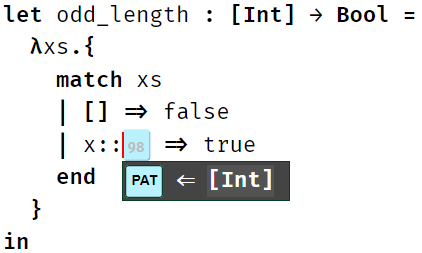
\includegraphics[scale=0.5]{imgs/maybe_exhaustive.png}
}
\hfill
  \subfloat[Must not be exhaustive.\label{fig:not-exhautive}]{
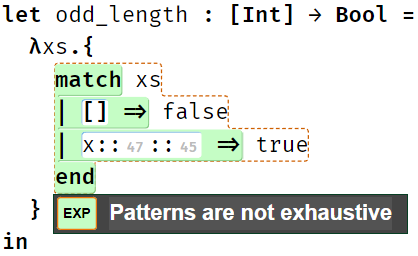
\includegraphics[scale=0.5]{imgs/not_exhaustive.png}
}
  \caption{Exhaustiveness Checking in Incomplete Match Expressions}
  \label{fig:exhaustiveness}
\end{figure}

It is possible for a match expression with pattern holes to be known to be not exhaustive. 
We see in \autoref{fig:not-exhautive} that again the pattern of the match expression contains a hole. 
However, there is no way to fill in this hole such that the branches are exhaustive following the same reasoning as before. Regardless of how the hole is filled, this pattern will not match lists with fewer than two elements. 
Hazel displays a warning message to the programmer in this situation because it is known that the match expression must not be exhaustive.

Next, let us discuss redundancy checking when pattern holes are present. 
Similar to exhaustiveness checking, we consider if there is a way that the pattern holes could be filled such that the match expression might not be redundant. 
If there is, we say that the match expression may or may not be redundant. 
If there is no such way to fill the holes, then the expression must be redundant.

Let us consider the example shown in \autoref{fig:redundancy}. 
In \autoref{fig:may-redundant}, we see that there is a pattern hole in the second branch of the match expression. 
It is possible to fill in this hole in a way that would not make the branches redundant, such as the empty list pattern, \texttt{[]}. 
However, it is also possible that the hole could be filled in a way that causes a redundancy, such as the cons pattern \texttt{y::xs}. 
This cons filling would make the third branch redundant since there is no expression that would match the third branch that would not first match with the second branch.
Again, similarly to exhaustiveness checking, since the branches are not known to be redundant, Hazel does not display a warning message to the programmer.

\begin{figure}[h]
  \centering
    \subfloat[May or may not be redundant. \label{fig:may-redundant}]{
    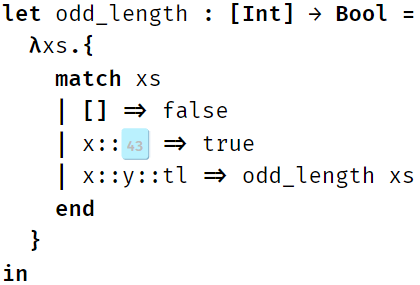
\includegraphics[scale=0.5]{imgs/maybe_redundant.png}
    } 
    \hfill
  \subfloat[Must be redundant. \label{fig:must-redundant}]{
  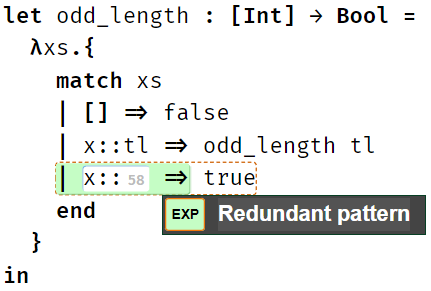
\includegraphics[scale=0.5]{imgs/redundant.png}
  }%
  \caption{Redundancy Checking in Incomplete Match Expressions}
  \label{fig:redundancy}
\end{figure}

Now let us look at \autoref{fig:must-redundant}. 
Here we see a situation where there is a hole in the pattern for the third branch of the match expression. 
However, there is no way to fill the hole such that this third branch would not be redundant. 
This is because the first and second branches will match all empty and non-empty lists, respectively, meaning that no expression would be matched by the third branch that would not already have been matched in prior branches.
Thus we can see that this third rule must be redundant, and Hazel shows a warning on the redundant rule.

Now that we have introduced the intuition for exhaustiveness and redundancy checking, we move to live evaluation of match expressions in the presence of pattern and expression holes. 
We first look at the situation where there are expression holes. 
We see in \autoref{fig:exp-hole} that the argument to \texttt{has\_odd\_length} has a hole. 
During evaluation, Hazel checks which pattern matches this expression. 
We can determine that the first branch does not match since regardless of how the expression hole is filled, the argument list is not empty. 
Similarly, we can also determine that the second branch does not match because regardless of how the expression hole is filled, the list is at least of length two. 
When checking the third branch, we see that we have a pattern that matches a list of at least two elements.
As just stated, our input list with a hole will have at least two elements regardless of how that hole is filled.
Thus, Hazel can take this third branch, binding \texttt{xs} to hole \todo{fill in with ending hole number}. 
The expression is then evaluated, applying \texttt{has\_odd\_length} again, this time with argument hole \todo{fill in with ending hole number}. 
When we evaluate to the match again, we cannot determine which branch to take since the empty hole may match (but also may not) the first rule. 
Therefore, our evaluation stops. Hazel indicates to the programmer which branch evaluation stopped on by greying out all previous branches, as can be seen on the bottom of \autoref{fig:exp-hole}. \todo{Screenshot doesn't have anything greyed out...}

\begin{figure}[h]
\centering
\subfloat[Pattern matching with expression  holes.\label{fig:exp-hole}]{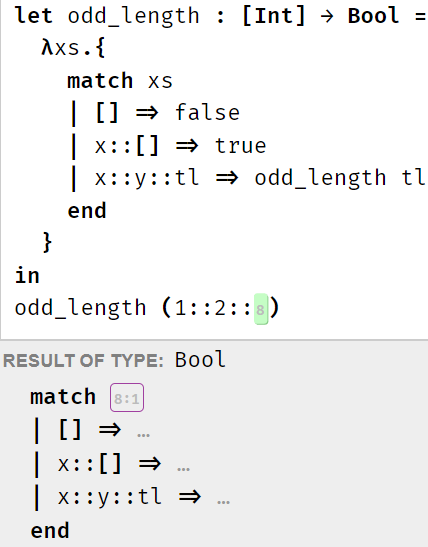
\includegraphics[scale=0.47]{imgs/pat_match_exp_holes.png}}
\hfill
\subfloat[Pattern matching with pattern holes.\label{fig:pat-hole}]{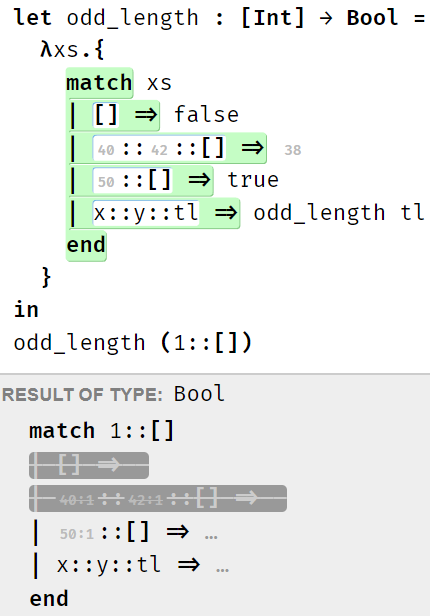
\includegraphics[scale=0.47]{imgs/pat_match_pat_holes.png}}
  \caption{Pattern Matching with Holes}
  \label{fig:evaluation-ex}
\end{figure}

Next we look at the situation where there are pattern holes during evaluation. 
We see in \autoref{fig:pat-hole} that we have a hole in the patterns of the match expression. 
Hazel evaluates down to the match expression, branching on the function argument \texttt{1::[]}. 
This argument does not match the pattern of the first branch, so evaluation moves to the second. 
While the pattern of the second branch has a hole, we are still able to determine that this branch does not match. 
We can do this because there is no way to fill in hole \todo{fill in with ending hole number} such that that pattern will match a list with two elements. 
Hazel uses hole based filling, so the only patterns that can fill in the pattern hole have to be for the head of the list, and the head of a list is only one element. 
Evaluation therefore moves to the third branch. 
Here evaluation stops since in this scenario of a pattern hole, we cannot determine if the expression we are branching on will match this pattern. \todo{This does not match up with the screenshot (is there supposed to be two elements in the input list and a hole somewhere in the third pattern}
Therefore, evaluation stops on the third branch as indicated in the Hazel UI. \todo{Again, no indication right now...}
